\documentclass[../main.tex]{subfiles}

\begin{document}

\begin{theorem}[Hartogs phenomenon]
$\Omega\subseteq\mathbb C^n$ is open, $n>1$, $K\subseteq\Omega$ is compact, $f\in\mathcal O(\Omega\setminus K)$, then there exists $g\in\mathcal O(\Omega)$ such that $f\equiv g$ on $\Omega\setminus K$
\end{theorem}

\begin{remark}
Holomorphic functions with more than one variable don't have isolated poles. The zero set of a holomorphic function with more than one variable is not contained in a compact set
\end{remark}

\begin{proof}
$\varphi\in C^\infty_0(\Omega)$ such that $\varphi\equiv1$ on a neighborhood of $K$, $v=\bar\partial(1-\varphi)f=-f\bar\partial\varphi\in(C^\infty_0)_{0,1}(\mathbb C^n)$, $\bar\partial v=\bar\partial(-f\bar\partial\varphi)=-f\bar\partial\bar\partial \varphi=0\Rightarrow\exists_1 u\in C^\infty_0(\mathbb C^n)$ such that $\bar\partial g=-f\bar\partial\varphi-\bar\partial u=0\Rightarrow g\in\mathcal O(\Omega)$, on $\partial\Omega$, $1-\varphi\equiv1$, $u\equiv0$, then use the identity theorem
\end{proof}

\begin{definition}
$\Omega$ is a domain of holomorphy if there exists $f\in\mathcal O(\Omega)$ such that $f$ doesn't extend to $\Omega'$ where $\Omega\subsetneqq\Omega'\subseteq\mathbb C^n$
\end{definition}

\begin{question}
Characterize the domains of holomorphy
\end{question}

Consider $f(z)=\sum_{\alpha\geq0}a_{\alpha}z^\alpha$, $D$ is the domain of convergence satisfies
\begin{enumerate}
\item $D$ is \textit{polycircular}, i.e. $z\in D\Rightarrow(e^{i\theta_1}z_1,\cdots,e^{i\theta_n}z_n)\in D$
\item $D$ is \textit{log-convex}, i.e. if $z^1,z^2\in D$, then $(z^1)^\beta(z^2)^{1-\beta}\in D$, $0<\beta<1$, here $z^\beta=(z_1^\beta,\cdots,z_n^\beta)$, note that $a^\alpha b^{1-\alpha}\leq\alpha a+(1-\alpha)b$ is Young's inequality
\end{enumerate}

\begin{definition}
$D$ is \textit{Reinhardt}\index{Reinhardt} if $D$ is polycircular. $D$ is \textit{log-convex Reinhardt} if $D$ also satisfies
\begin{itemize}
\item $D^*=\log|D|=\{(t_1,\cdots,t_n)\in\mathbb R^n|(e^{t_1},\cdots,e^{t_n})\in D\}$ is a convex set of $\mathbb R^n$ and $D^*+(\mathbb R_-)^n\subseteq D^*$
\end{itemize}
If $D$ is Reinhardt, then $\hat D=\cap\{\tilde D\text{ Reinhardt and log convex, }D\subseteq\tilde D\}$ is the log-convex cover of $D$
\end{definition}

\begin{theorem}
If $0\in D\subseteq\mathbb C^m$ is connected Reinhardt, $f\in\mathcal O(D)$, then there exists $g\in\mathcal O(\hat D)$ such that $g|_D=f$
\end{theorem}

\begin{proof}
$f(z)=\sum_{\alpha\geq0}a_{\alpha}z^\alpha$ in $D(0,\delta)^m$ extends to $D$, use the fact that the domain of absolute convergence of $\sum_{\alpha\geq0}a_{\alpha}z^\alpha$ is a log convex Reinhardt domain containing $D$
\end{proof}

\begin{definition}
Domain $\Omega\subseteq\mathbb C^n$ is a domain of holomorphy if there are no open sets $\Omega_1$, $\Omega_2$ such that
\begin{itemize}
\item $\varnothing\neq\Omega_1\subseteq\Omega_2\cap\Omega$\begin{center}
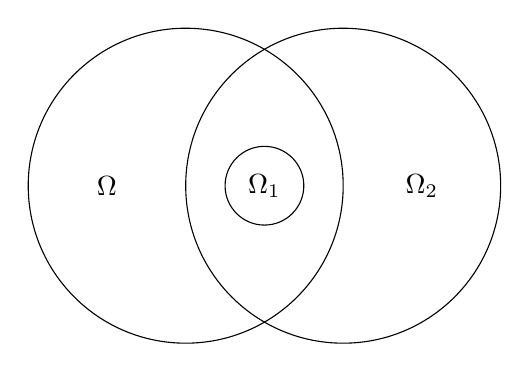
\begin{tikzpicture}
\draw (-1,0) circle (2);
\draw (1,0) circle (2);
\draw (0,0) circle (0.5);
\node at (-2,0) {$\Omega$};
\node at (2,0) {$\Omega_2$};
\node at (0,0) {$\Omega_1$};
\end{tikzpicture}
\end{center}
\item For any $f\in\mathcal O(\Omega)$, there exists $g\in\mathcal O(\Omega_2)$ such that $f|_{\Omega_1}=g|_{\Omega_1}$
\end{itemize}
\end{definition}

\begin{remark}
Local property of $\partial\Omega$, to rule out anomalies from slit type domain
\begin{center}
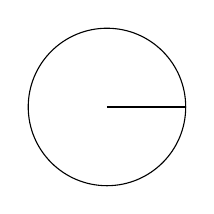
\begin{tikzpicture}
\draw (0,0) circle (1);
\draw (0,0)--(1,0);
\end{tikzpicture}
\end{center}
\end{remark}

\begin{definition}
$K\subseteq\Omega$ is compact, its holomorphically convex hull is
\[\hat K_\Omega=\left\{z\in\Omega\middle||f(z)|\leq\sup_K|f|,\forall f\in\mathcal O(\Omega)\right\}\]
\end{definition}

\begin{note}
$K\subseteq\hat K_\Omega$
\end{note}

\begin{remark}
$\hat K_\Omega$ is contained in the convex hull of $K$
\end{remark}

\begin{proof}
Let $L(\mathbb C^n)$ be the set of complex linear functionals of $\mathbb C^n$, $L_\mathbb{R}(\mathbb C^n)$ be the set of real linear funcitonals of $\mathbb C^n$, $\operatorname{Re}L(\mathbb C^n)=L_{\mathbb R}(\mathbb C^n)$
\begin{align*}
\operatorname{convex}(K)&\xequal{\text{Hahn-Banach}}\{z\in\Omega|\Lambda(z)\leq\sup_K\Lambda,\Lambda\in L_{\mathbb R}(\mathbb C^n)\} \\
&=\{z\in\Omega|e^{\Lambda(z)}\leq e^{\sup_K\Lambda(z)},\Lambda\in L_{\mathbb R}(\mathbb C^n)\} \\
&=\{z\in\Omega|e^{\operatorname{Re}\beta(z)}\leq e^{\sup_K\operatorname{Re}\beta(z)},\beta\in L(\mathbb C^n)\} \\
&=\{z\in\Omega||e^{\beta(z)}|\leq\sup_K|e^{\beta}|,\beta\in L(\mathbb C^n)\}
\end{align*}
\end{proof}

\begin{remark}
$K\subseteq\Omega$ is compact and convex, then $\widehat{\partial K_{\Omega}}=K$. Maximal principle: $K\subseteq\widehat{K_\Omega}=\widehat{\partial K_\Omega}$
\end{remark}

\begin{proof}
$\widehat{\partial K_{\Omega}}\subseteq\operatorname{convex}(\partial K)\xequal{\text{Milman-Kreim}}K$
\end{proof}

\begin{lemma}\label{Lemma 2.5.3}
Let $D$ be a polydisk centered at $0\in\mathbb C^n$, $\Delta_\Omega^D(z)=\sup\{r>0,s.t. z+rD\subseteq\Omega\}$ is the "weighted" $L^\infty$ distance of $z$ to $\partial\Omega$. $r=\inf_{z\in K}\Delta_\Omega^D(z)>0$, $K\subseteq\Omega$ is compact. Let $\xi\in\hat K_\Omega$, if $u\in\mathcal O(\Omega)$, then the power series expansion of $u$ at $\xi$
\[f(z)=\sum_\alpha\frac{1}{\alpha!}\frac{\partial^\alpha u(\xi)}{\partial\xi^\alpha}(z-\xi)^\alpha\]
is convergent for any $z\in\xi+rD$
\end{lemma}

\begin{proof}
$\sup_Ku(z)\leq M$, then $|\frac{\partial^\alpha u(z)}{\partial z^\alpha}|\leq\frac{\alpha! M}{(r-\epsilon)^{|\alpha|}}$ for any $z\in K$, $\Rightarrow |\frac{\partial^\alpha u(\xi)}{\partial \xi^\alpha}|\leq\frac{\alpha! M}{(r-\epsilon)^{|\alpha|}}$, then $|u(z)|=|\sum\frac{1}{\alpha!}\frac{\partial^\alpha u(\xi)}{\partial\xi^\alpha}(z-\xi)^\alpha|\leq\sum_\alpha\frac{M}{|r-\epsilon|^\alpha}(z-\xi)^\alpha\xRightarrow{\text{Abel's criterion}}$ absolutely convergent for $z\in\xi+(r-\epsilon)D$, then let $\epsilon\searrow0$
\end{proof}

\begin{definition}
$\Omega\subseteq\mathbb C^n$ is holomorphically convex if for any $K\subseteq\Omega$ compact, $\hat K_\Omega$ is also compact
\end{definition}

\begin{theorem}
$\Omega\subseteq\mathbb C^n$ is open, the following are equivalent
\begin{enumerate}[label=(\roman*)]
\item $\Omega$ is a domain of holomorphy
\item $K\subseteq\Omega$ compact $\Rightarrow$ $\hat K_\Omega\subseteq\Omega$ is compact, i.e. $K\subseteq\Omega$ is holomophically compact
\item $\exists f\in\mathcal O(\Omega)$ such that doesn't extend over any point $\in\partial\Omega$ holomorphically
\end{enumerate}
\end{theorem}

\begin{proof}
(i)$\Rightarrow$(ii): $r=\inf_{z\in K}\Delta^D_\Omega(z)>0\xRightarrow{Lemma \ref{Lemma 2.5.3}}\hat K_\Omega+rD\subseteq \Omega$ \par
(iii)$\Rightarrow$(i): Trivial \par
(ii)$\Rightarrow$(iii): Let $M$ be a dense, countable set in $\Omega$. Let $\xi,\cdots,\xi_n,\cdots$ be a sequence containing each element of $M$ infinitely many times. Let $K=K^1\subseteq K^2\subseteq\cdots\subseteq\Omega$ is another compact exhaustion of $\Omega$, by (ii), we have $\hat K^1_\Omega\subseteq\hat K^2_\Omega\subseteq\cdots\subseteq\Omega$ is another compact exhaustion of $\Omega$. $D_\xi=\xi+\Delta^D_\Omega(\xi)D\subseteq\Omega$. For any $\xi_j$, $\exists z_j\in D_{\xi_j}$ such that $z_j\in\hat K^j_\Omega$ because it's compact. $\exists f\in\mathcal O(\Omega)$ such that $\begin{cases}
|f_j(z_j)|=1 \\
\sup_{z\in K_j}|f_j(z)|<1-\epsilon
\end{cases}\xRightarrow{\text{manipulate power}}\begin{cases}
f_j(z_j)=1 \\
\sup_{z\in K_j}|f_j(z)|<\frac{1}{2^j}
\end{cases}$. $f(z)=\prod_{j=1}^\infty(1-f_j)^j$. Claim: $f\in\mathcal O(\Omega)$. $z\in\Omega\Rightarrow z+\epsilon D\subseteq K_j$ for all $j\geq j_0$. $\log\prod_{j\geq j_0}(1-f_j)^j=\sum_{j\geq j_0}j\log(1-f_j)$, thus $|\log(1-f_j(z))|\leq C|f_j(z)|$, then $\sum_{j\geq j_0}j|\log(1-f_j)|\leq\sum_{j\geq j_0}jC|f_j|\leq C\sum_{j\geq j_0}\frac{j}{2^j}<\infty$
\end{proof}

\begin{exercise}
$f$ is not identically zero, but $f(z_j)=0$, $\frac{\partial^\alpha f}{\partial z^\alpha}(z_j)=0$, for all $|\alpha|\leq j$. Assume $f$ extends across $\partial\Omega$, contradiction
\end{exercise}

\begin{example}
$\Omega\subseteq\mathbb C^n$ convex and open $\Rightarrow$ $\Omega$ is a domain of holomorphy. Pf: Only need to show $K\subset\subset\Omega\Rightarrow\hat K_\Omega\subset\subset\Omega$. $\hat K_\Omega\subset\operatorname{convex}(K)\subseteq\Omega\Rightarrow\hat K_\Omega$ is closed and bounded $\Rightarrow\hat K_\Omega$ is compact \par
Reinhardt domains: $0\in\Omega$ is a connected Reinhardt domain, $\Omega^*=\{\xi\in\mathbb R^n|(e^{\xi_1},\cdots,e^{\xi_n})\in\Omega\}$. $\Omega$ is log convex $\Leftrightarrow$ $\Omega^*$ is convex, and for any $\xi\in\Omega^*$, $\eta_j\leq \xi_j\Rightarrow\eta\in\Omega^*$
\end{example}

\begin{theorem}
$\Omega$ is a Reinhardt domain, tthen the following are equivalent
\begin{enumerate}[label=(\roman*)]
\item $\Omega$ is a domain of holomorphy
\item $\Omega$ is log-convex
\end{enumerate}
\end{theorem}

\begin{proof}
(i)$\Rightarrow$(ii): $\exists f\in\mathcal O(\Omega)$ that does not extend through any boundary point $\Rightarrow$ power series expansion of $f$ at $0$ absolutely converges exactly on $D$ $\Rightarrow$ $D$ is log-convex \par
(ii)$\Rightarrow$(i): Take $K\subset\subset\Omega$, $\exists\xi^j$ such that $K\subseteq\cup_{j=1}^kD(0,\xi^j_1)\times\cdots\times D(0,\xi^j_n)$, $z\in K\Rightarrow |z_1|^{\alpha_1}\cdots|z_n|^{\alpha_n}\leq\sup_{1\leq j\leq k}|\xi_1^j|^{\alpha_1}\cdots|\xi^j_n|^{\alpha_n}$ which holds for $\alpha\in\mathbb Q_+^n$, by density, it also holds for $\alpha\mathbb R^n_+$, thus also holds for $z\in\hat K_\Omega$, assume that $z_1,\cdots,z_j\neq0$, $z_{j+1}=\cdots=z_n=0$. Take $\alpha=(\alpha_1,\cdots,\alpha_j,0,\cdots,0)$, $|z_1|^{\alpha_1}\cdots|z_j|^{\alpha_j}\leq\sup_{1\leq l\leq k}(\alpha_1\log|\xi^l_1|+\cdots+\alpha_j\log|\xi^l_j|)$. claim (HW): $(\log|z_1|,\cdots,\log|z_j|)$ is in the convex hull of vectors $(\log\eta_1,\cdots,\log\eta_j)$ such that $\eta_j\leq\xi^l_j$ for some $l\in\{1,\cdots,k\}$
\end{proof}

\begin{lemma}
$f\in\mathcal O(\Omega)$ such that $|f(z)|\leq\Delta^D_\Omega(z)=\sup\{r>0|z+rD\subseteq\Omega\}$, $z\in K$, $\xi\in \hat K_\Omega$, $u\in\mathcal O(\Omega)$, then the power series expansion of $u$ near $\xi$ absolutely converges in $\xi+|f(\xi)|D$
\end{lemma}

\end{document}